\documentclass{article}

% Language setting
% Replace `english' with e.g. `spanish' to change the document language
\usepackage[english]{babel}

% Set page size and margins
% Replace `letterpaper' with `a4paper' for UK/EU standard size
\usepackage[letterpaper,top=2cm,bottom=2cm,left=3cm,right=3cm,marginparwidth=1.75cm]{geometry}

% Useful packages
\usepackage{amsmath}
\usepackage{graphicx}
\usepackage[colorlinks=true, allcolors=blue]{hyperref}

% \title{Your Paper}
% \author{You}

\begin{document}
% \maketitle

% \begin{abstract}
% \end{abstract}


\section{Methods}

To simulate membranes, we used a triangular mesh. Each timestep, the vertex positions are updated based on the discrete membrane Hamiltonian using different integration schemes. Our simulator calculates the gradients and Hessians of the Hamiltonian based on the geometric information around the vertex. To model the membrane we use the Helfrich Hamiltonian, its most general expression is.
\begin{equation}
    H_\text{Helfrich} =\displaystyle\int_{\mathcal{M}} \left( \cfrac{\kappa}{2}(2H-c_0)^2 +\kappa_G K+ \sigma\right)dA
\end{equation}
Where $H$ and $K$ correspond to the scalar mean curvature and Gaussian curvature respectively.The constant $c_0$ corresponds to the spontaneous curvature. The constants $\kappa,\kappa_G$ and $\sigma$ are the bending rigidity, the Gaussian modulus and surface tension. 
For the simulations we need to calculate the discrete gradients of the energy.Therefore we need to discretize the integrals. Our discretization scheme consist of using the dual area of each vertex and using local information to calculate the approximated quantity. For the squared mean curvature term, this looks like
\begin{equation}
    \cfrac{\kappa}{2}\displaystyle\int_{\mathcal{M}} (2H-c_0)^2 \approx \sum_{v_i\in V}(2\hat{H}-c_0)^2A_{v_i}
\end{equation}
At this point one needs to make the decision for the discrete scalar mean curvature $\hat{H}$ and the dual area $A_{v_i}$ expression. Based on [reference] one reliable discretization for the mean curvature is.
\begin{equation}
    \hat{H}_i = \sum_{e_{ij}\in N(v_i)}\cfrac{\ell_{ij}\varphi_{ij}}{4}
\end{equation}
where $e_{ij}$ is the edge that connects vertex $i$ and $j$ and $N(v_i)$ is the neighborhood of vertex $i$, $\ell_{ij}$ is the edge length of edge $ij$ and $\varphi_{ij}$ is the dihedral angle between the two faces that touch the edge $ij$. Its important to notice that since our mesh is manifold, every edge that is not in the boundary has only two faces touching it.




\section{Visualization}


\begin{figure}[htbp]
    \centering
    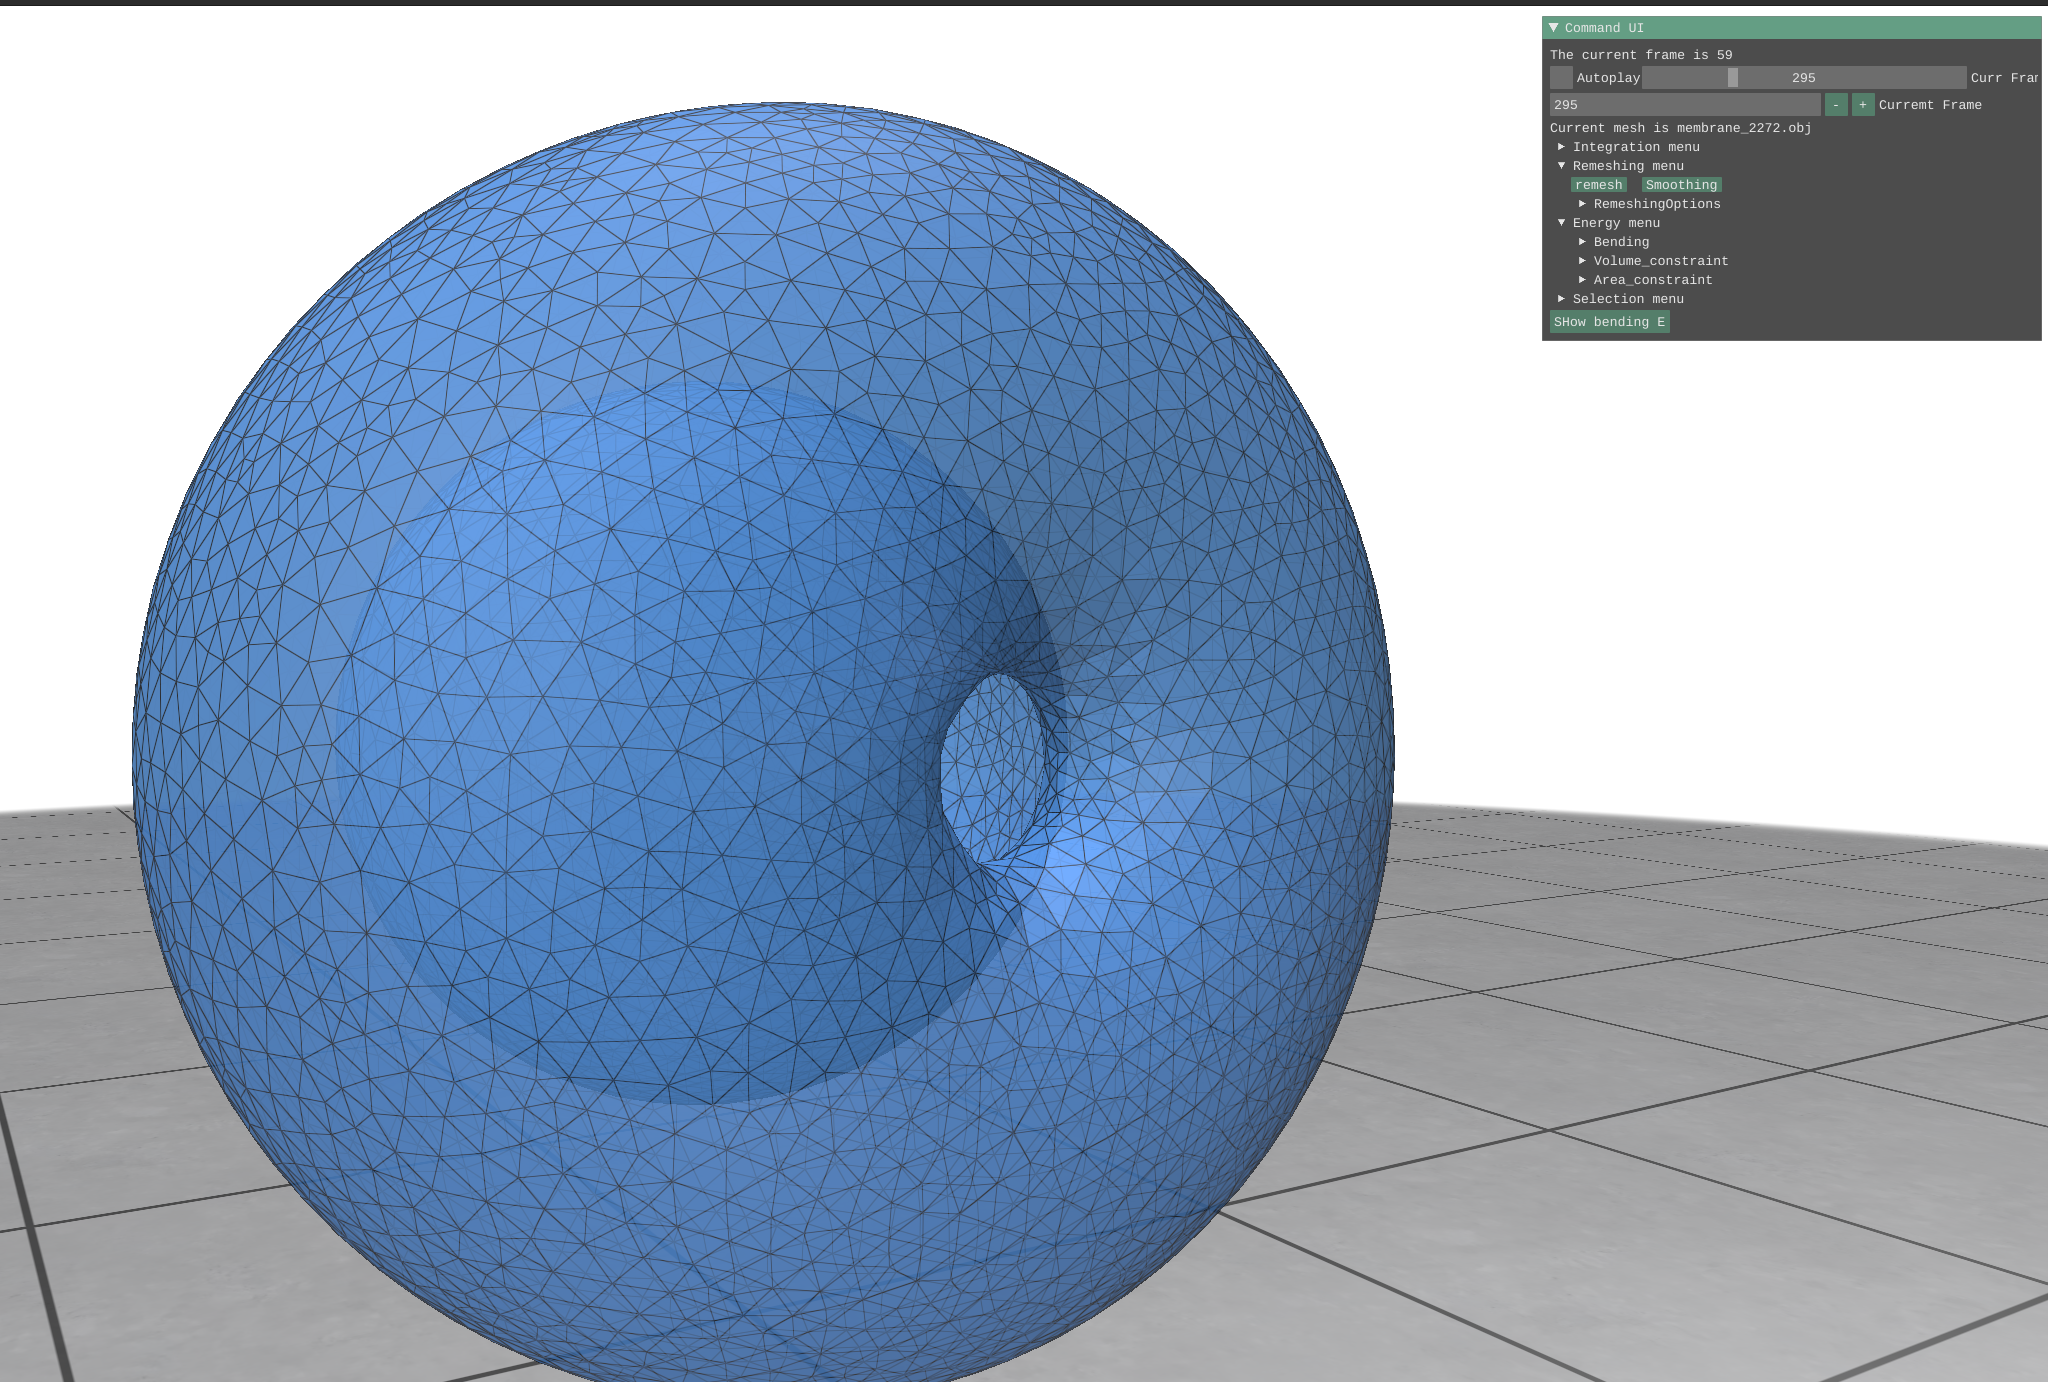
\includegraphics[width=10cm,keepaspectratio]{Polyscope1.png}
    \caption{Polyscope interface}
    \label{<label>}
\end{figure}

\end{document}
